\section{COMPONENTE HARDWARE}

El componente hardware se ha implementado utilizando dos lenguajes de programación; \emph{Wiring} para el microprocesador ATmega32u4, Python para el procesador \emph{Atheros AR9331}.

\subsection{Configurando el sistema}

El primer paso es configurar la placa de Arduino Yún para empezar a trabajar sobre ella. Para ello Yún corre una distribución de Linux llamada \emph{OpenWrt-Yun}, basado en \emph{OpenWrt}, la cual nos permite acceder vía \emph{ssh} o vía web para poder configurarla. 

La primera vez que se conecta Arduino Yún se crea una red sin encriptar para poder conectarnos a ella y poder configurarla, el nombre de la red tiene el formato \emph{ArduinoYun-XXXXXXXXXXXX}. Una vez conectados se accede al panel web de configuración a través de la url \emph{http://arduino.local} y se nos muestra la siguiente ventana:

\begin{figure}[H]
    \centering
    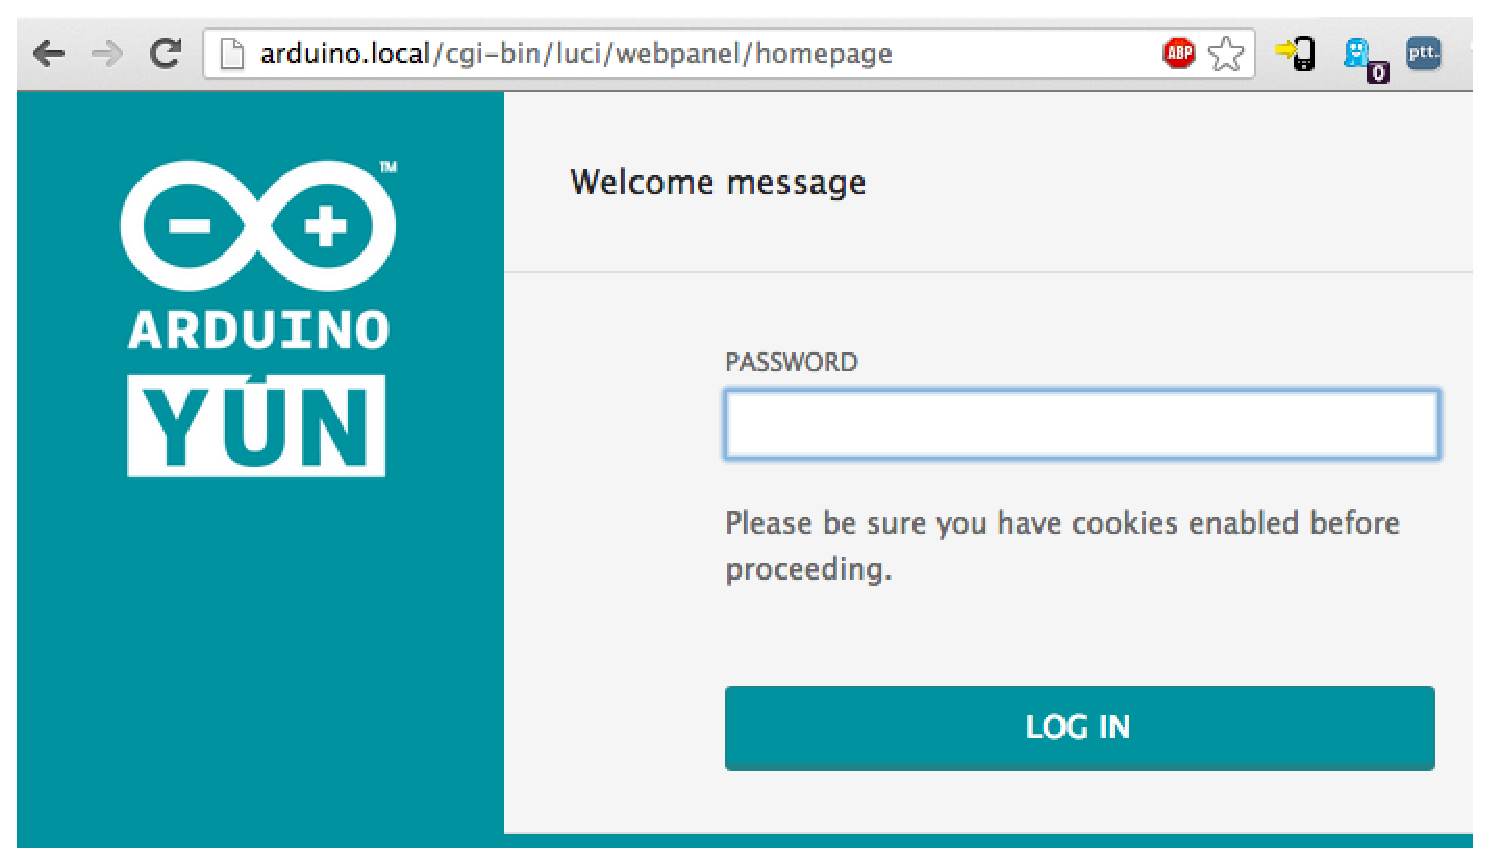
\includegraphics[keepaspectratio,width=0.6\textwidth]{YunWebPassword.eps}
    \caption{Arduino Yún Web Password}\label{fig:yun-web-password}
\end{figure}

La contraseña por defecto es \emph{Arduino} y nos permite acceder al panel de diagnóstico donde nos muestra información sobre la red WiFi y la conexión Ethernet. Además, nos permite acceder al panel de configuración:

\begin{figure}[H]
    \centering
    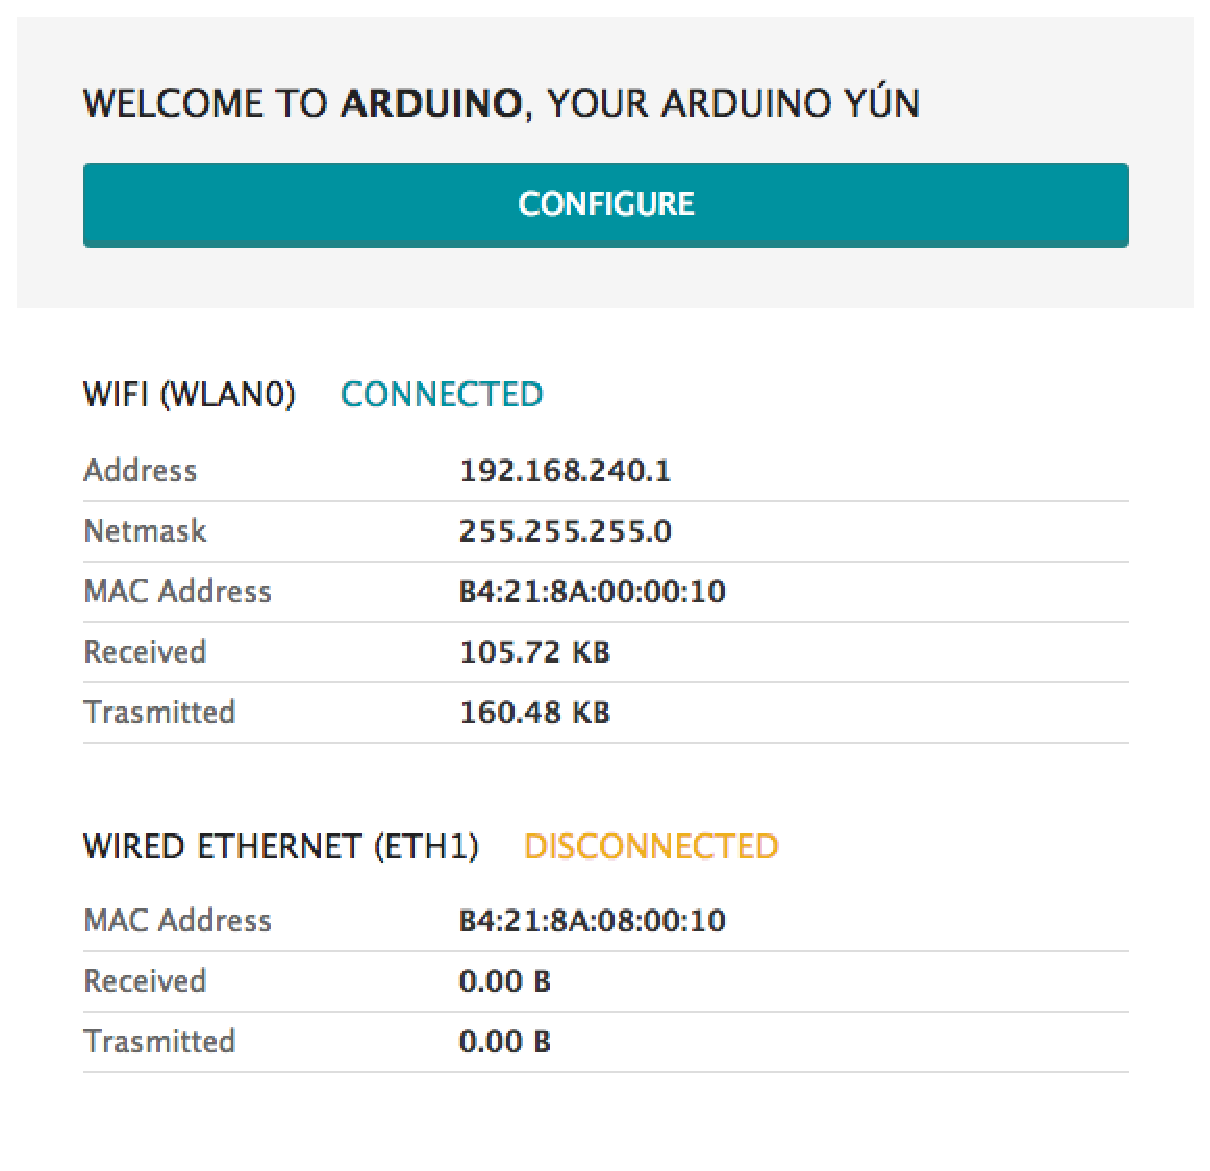
\includegraphics[keepaspectratio,width=0.6\textwidth]{YunWebDiagnostic.eps}
    \caption{Arduino Yún Web Diagnostic}\label{fig:yun-web-diagnostic}
\end{figure}

El panel de configuración nos permite nombrar nuestra placa Arduino, establecer una contraseña de acceso, configurar la zona horaria y por último, y lo más importante, decirle a que red WiFi debe conectarse.

\begin{figure}[H]
    \centering
    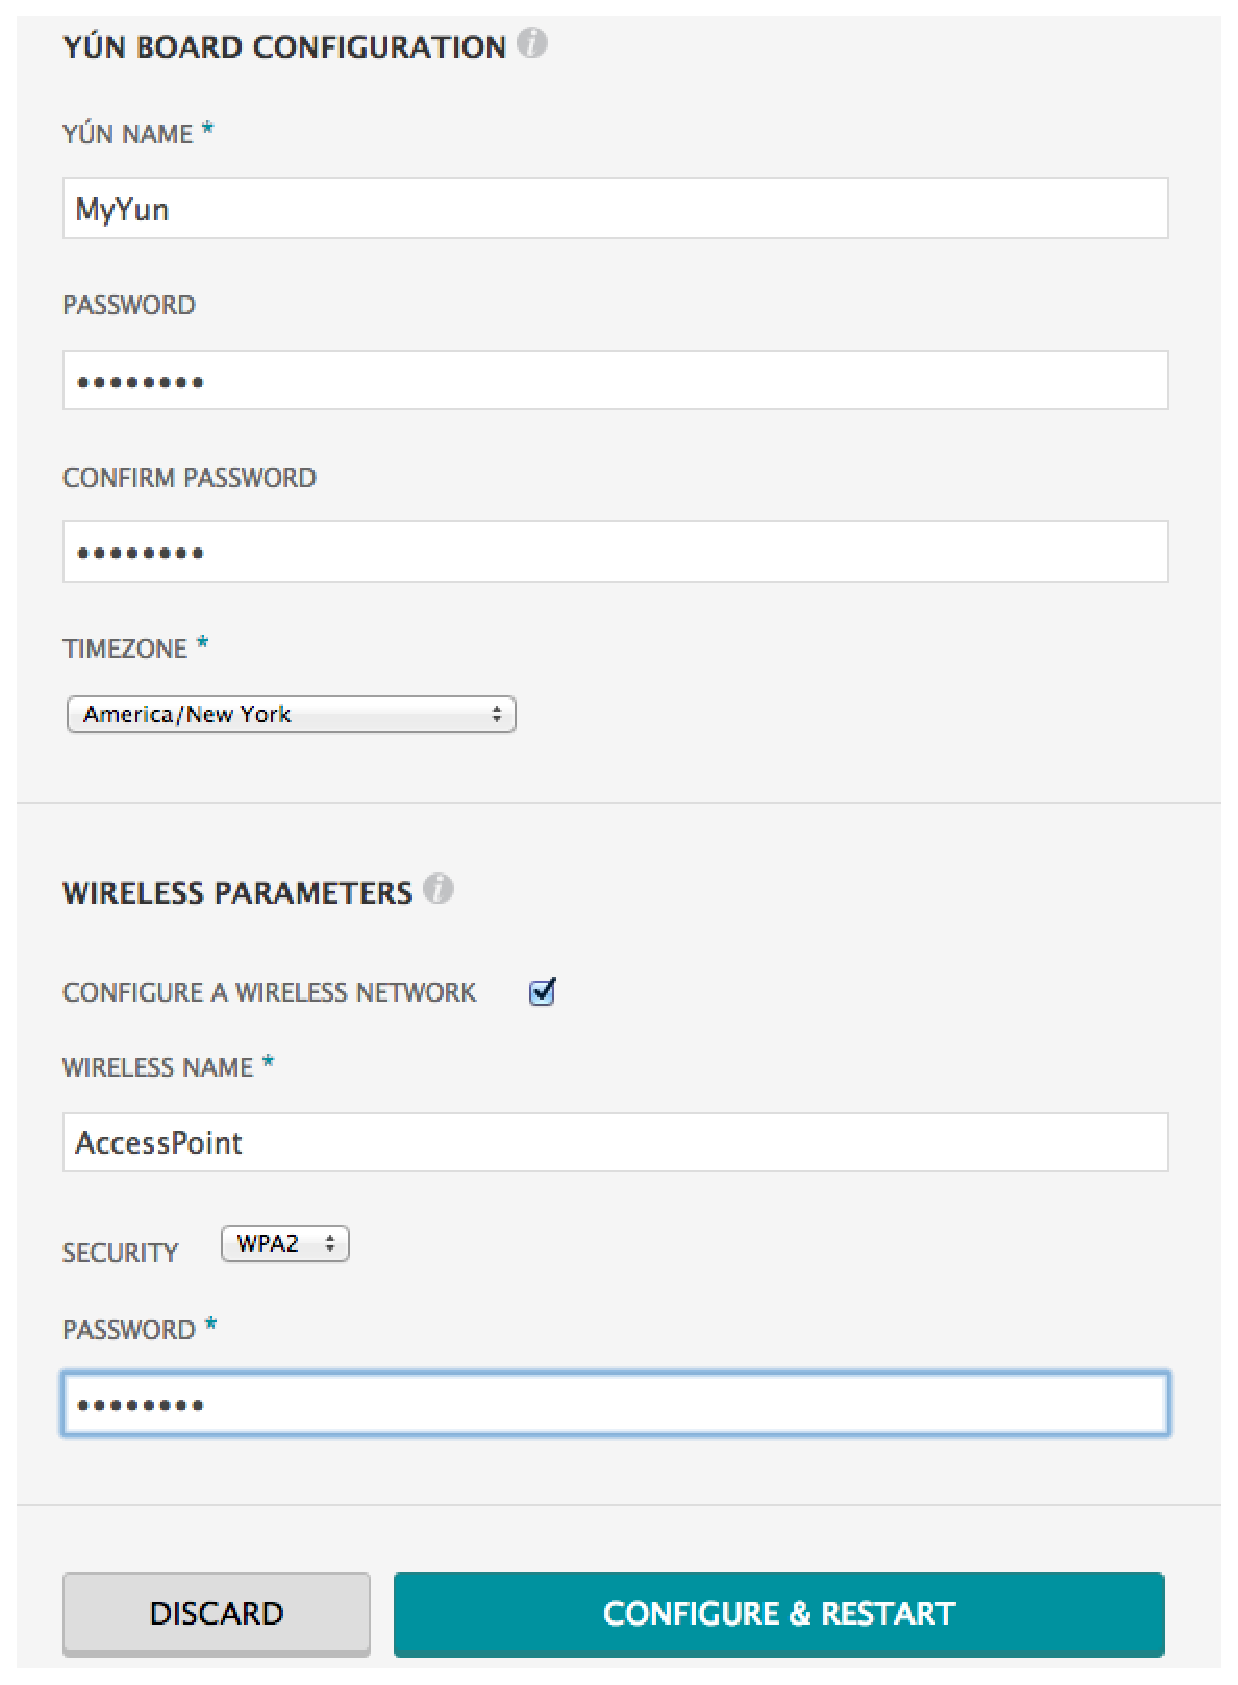
\includegraphics[keepaspectratio,width=0.6\textwidth]{YunWebConfig.eps}
    \caption{Arduino Yún Web Config}\label{fig:yun-web-config}
\end{figure}

Una vez se guarda la nueva configuración la distribución Linux se reinicia y automáticamente se conectará a la red WiFi que hayamos establecido, indicándonos que nos conectemos a la misma WiFi mediante la siguiente ventana:

\begin{figure}[H]
    \centering
    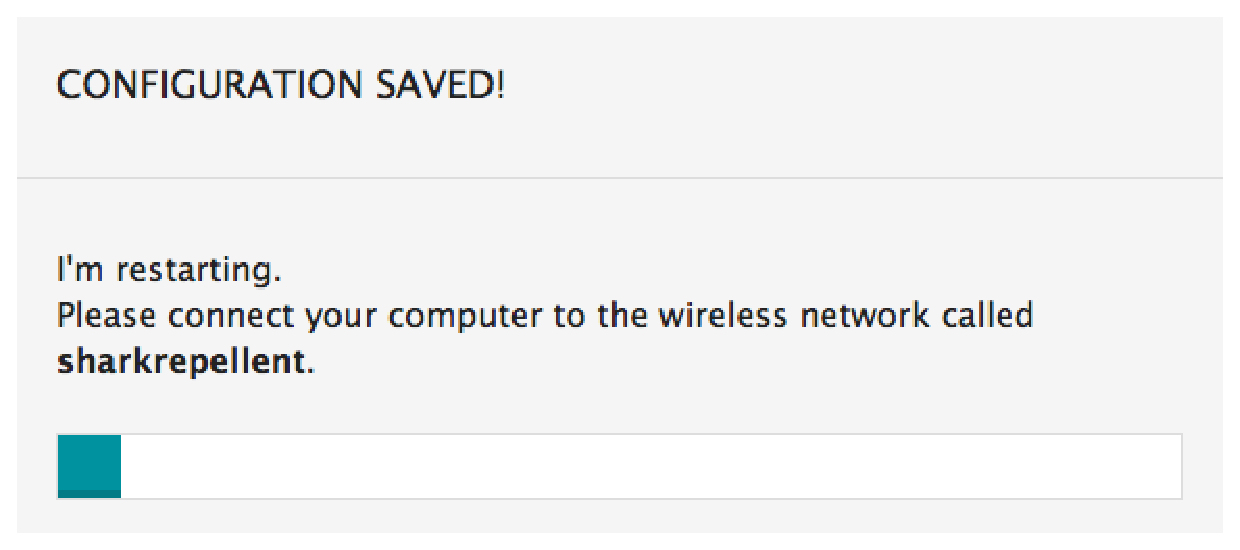
\includegraphics[keepaspectratio,width=0.6\textwidth]{YunRebooting.eps}
    \caption{Arduino Yún Web Rebooting}\label{fig:yun-web-rebooting}
\end{figure}

Pasado varios segundos automáticamente se nos volverá a conectar a la página de configuración de Arduino donde tendremos que introducir la nueva contraseña para acceder.

